\section{Membuat Aplikasi dengan Oracle APEX}
\paragraph{}Oracle Application Express (Oracle APEX) yang dulu disebut HTML-DB adalah sebuah framework yang berbasis pada sebuah database dedicated (sementara ini sampai versi terbaru masih dedicated untuk Oracle Db saja dan lisensi include dalam lisensi database), ini artinya apa bahwa engine aplikasi dibangun sepenuhnya didalam sebuah database. Bahkan untuk arsitektur Embedded PL/SQL Gateway seperti yang dipakai dalam Oracle XE dan Oracle 11G file image (library,css,theme,dll) disimpan didalam database metadata juga. Inilah hal yang berbeda dibandingkan framework yang lain. Berikut ini merupakan tata cara membuat suatu aplikasi di Oracle APEX:

\subsection{Tutorial masuk dan login Oracle APEX}
\begin{enumerate}
    \item Pertama, kita pilih menggunakan APEX Online atau APEX offline. Disini saya akan menggunakan APEX online dengan cara kunjungi website https://apex.oracle.com/en/
    \item Kedua, setelah masuk pada link akan muncul sepeti gambar dibawah ini kemudian silahkan sign in.
 \begin{center}
    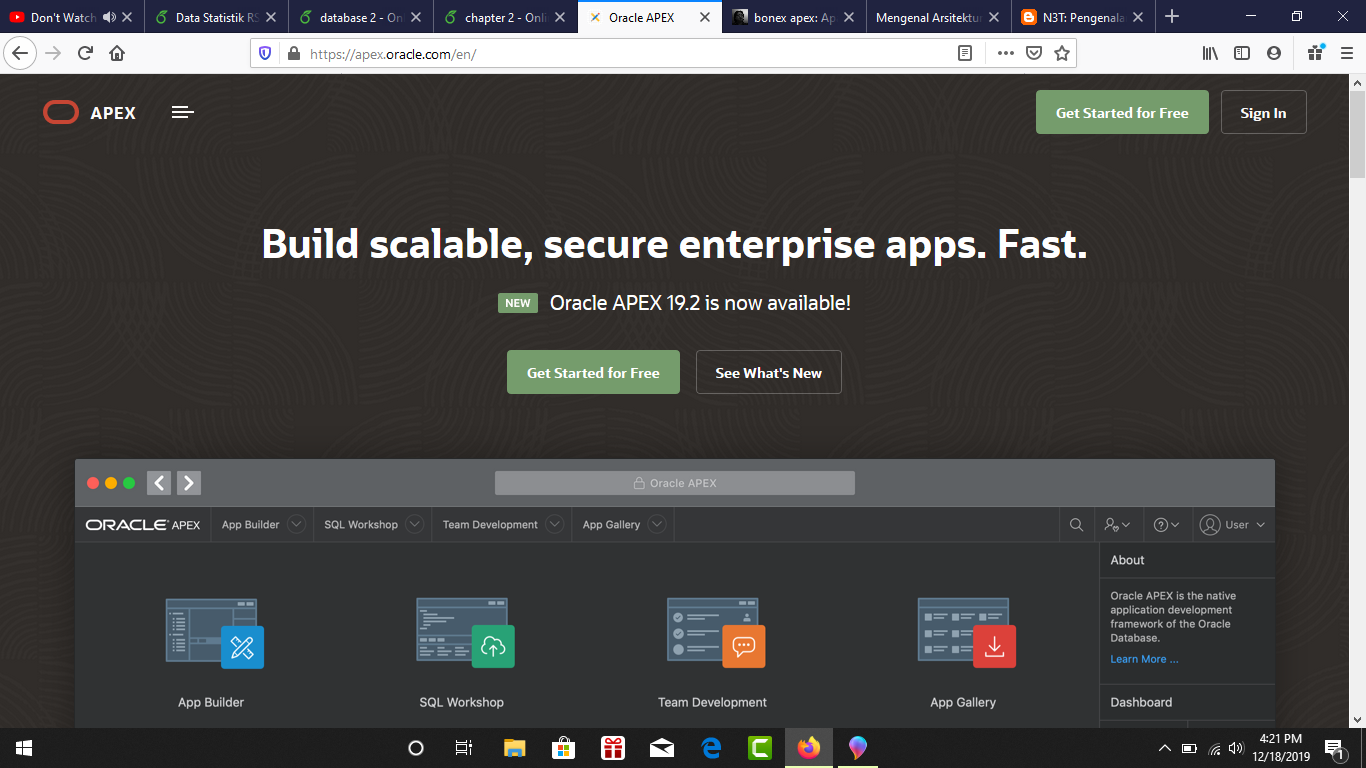
\includegraphics[width=10cm\textwidth]{gambar/1.png}
\end{center}
\newpage
    \item ketiga, pilih sign in jika kita sudah memiliki workspace. Lalu masukkan nama database yang telah dibuat, nama username dan password tetapi jika kita belum memiliki akun request workspace. Maka  ikuti langkah-langkah pada  form pendaftaran.  Ketika sudah kita telah selesai memasukkan nama database, username dan password yang telah dibuat.Maka kita bisa masuk dengan memasukkan data dengan benar sesuai data yang telah kita miliki.
    \begin{center}
    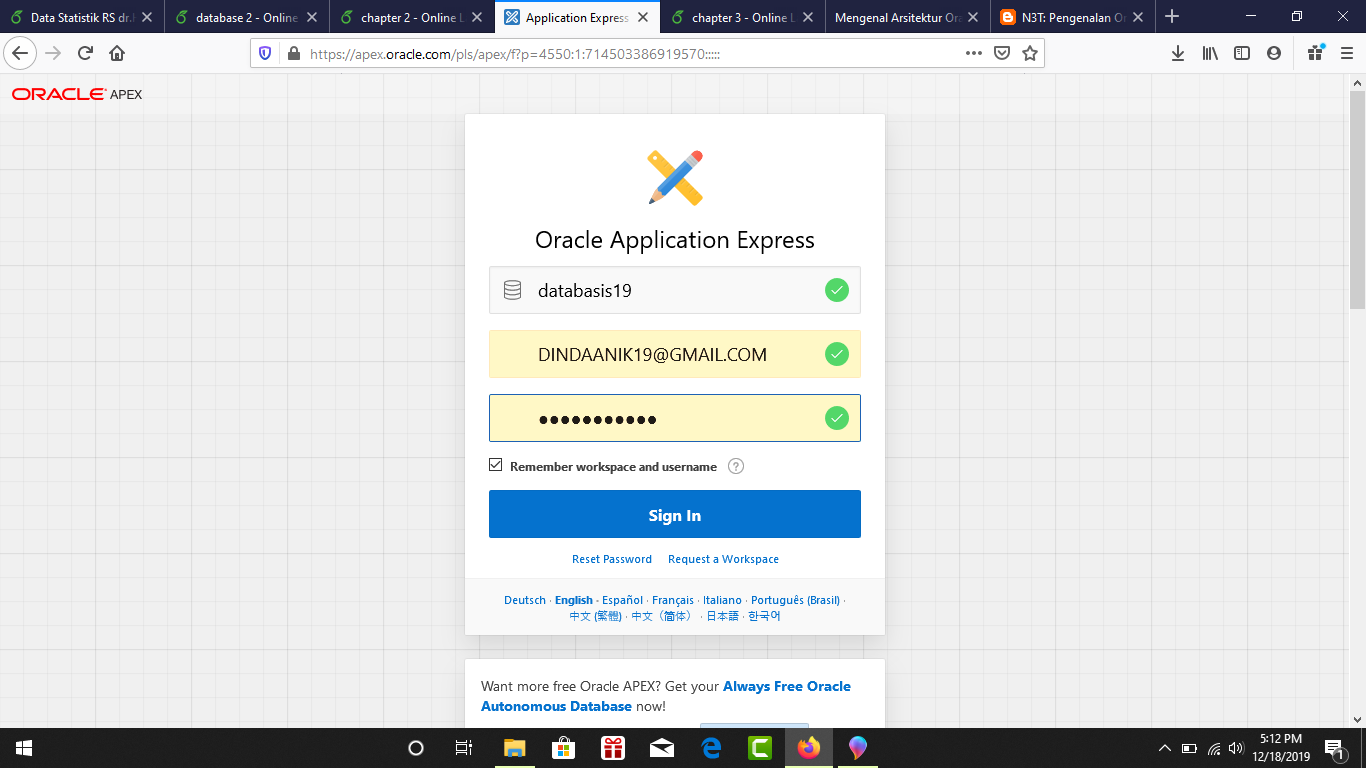
\includegraphics[width=10cm\textwidth]{gambar/2.png}
    \end{center}
\end{enumerate}

\subsubsection{Langkah-langkah Membuat Aplikasi Di Oracle APEX}
\begin{enumerate}
    \item Pertama, jika kita sudah menginstall aplikasi oracle apex atau sudah mendaftar di oracle apex online maka setelah itu akan masuk ke dalam aplikasi oracle apex.
     \begin{center}
    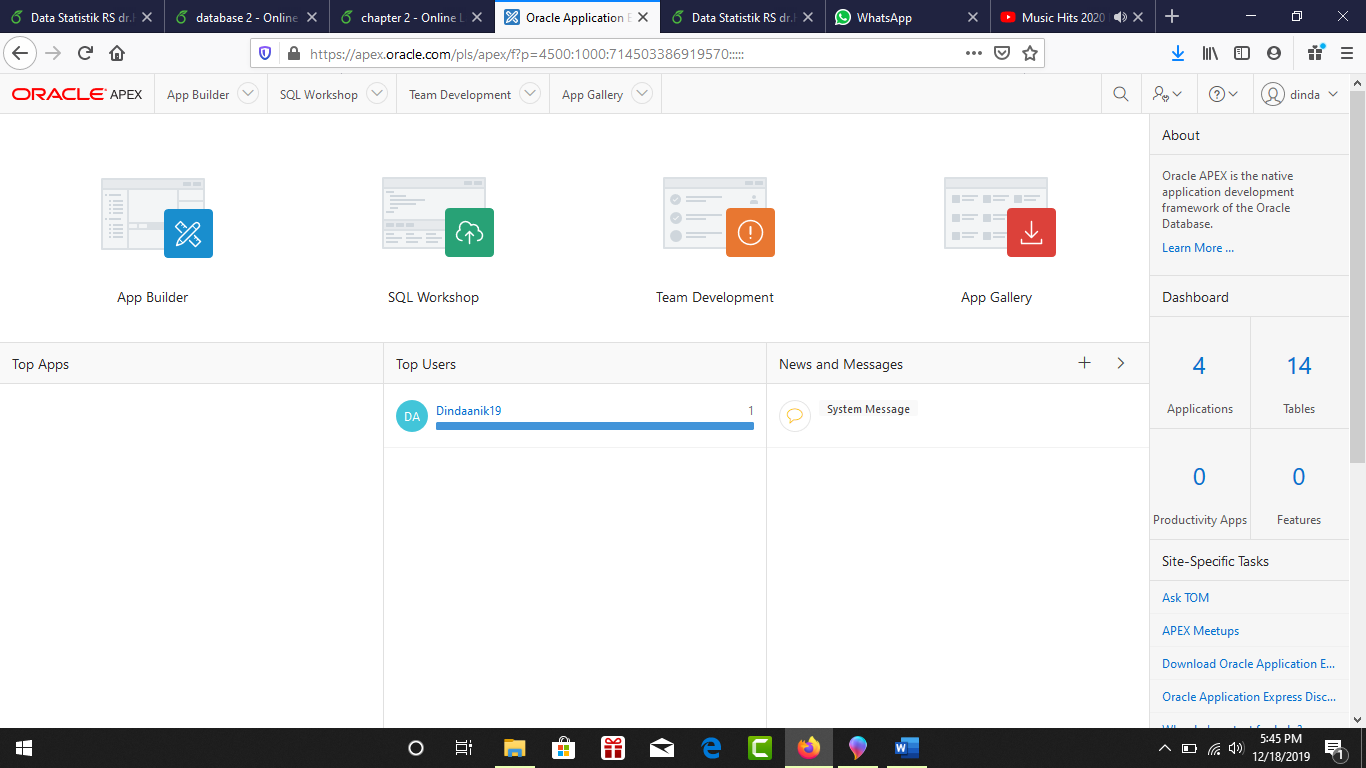
\includegraphics[width=10cm\textwidth]{gambar/3.png}
    \end{center}
    \item Kemudian, pilih sql workshop dan pilih sql command. Sql command digunakan untuk mengetikkan query yang akan digunakan dan dibuat.
    \item Langkah selanjutnya adalah pembuatan database yang dimulai dengan membuat table. Disini saya akan membuat aplikasi data statistik dari RS yang terdapat lima tabel yaitu pasien, dokter,obat,resep, dan diagnosa. Query yang diinputkan di sql command seperti berikut :
    \par \begin{enumerate}
        \item Table Pasien
        \par Table pasien yang mempunyai 6 kolom yaitu id pasien, nama pasien,tanggal lahir, alamat, no telp, dan jumlah periksa. Pada table ini yang menjadi primary keynya adalah id pasien.
         \begin{center}
    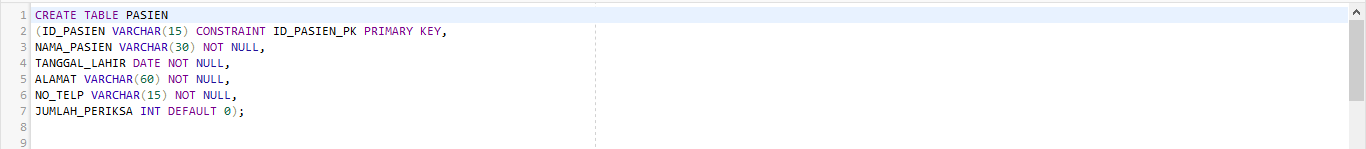
\includegraphics[width=10cm\textwidth]{gambar/4.png}
    \end{center}
    \item Table Dokter
    \par Table dokter yang mempunyai 6 kolom yaitu id dokter, nama dokter, alamat, no telp, keahlian, dan tarif. Pada table ini yang menjadi primary keynya adalah id dokter.
    \begin{center}
    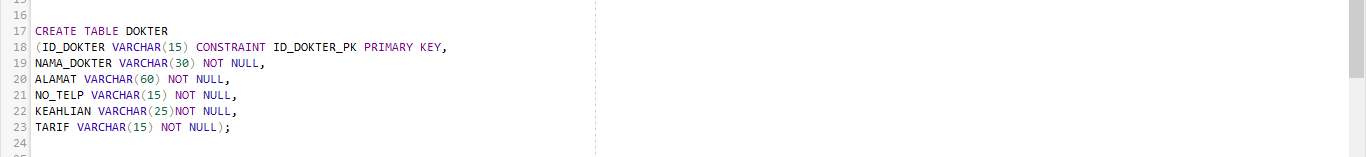
\includegraphics[width=10cm\textwidth]{gambar/5.png}
    \end{center}
    \item Table Obat
    \par Table obat yang mempunyai 4 kolom yaitu id-obat, nama-obat, kegunaan, dan harga-obat. Pada table ini yang menjadi primary keynya adalah id-obat.
    \begin{center}
    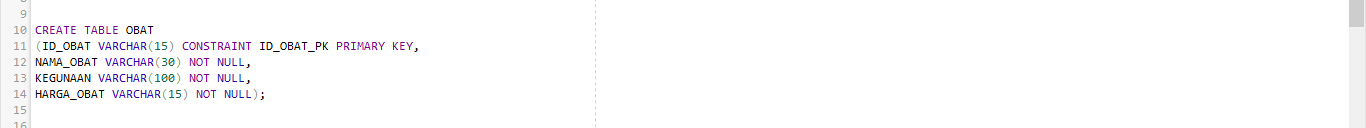
\includegraphics[width=10cm\textwidth]{gambar/6.png}
    \end{center}
    \item Table Resep
    \par Table resep yang mempunyai 5 kolom yaitu id resep, isi resep, id obat, id pasien, dan id dokter. Pada table ini yang menjadi primary keynya adalah id-resep dengan id pasien, id obat, dan id dokter sebagai foreign keynya.
    \begin{center}
    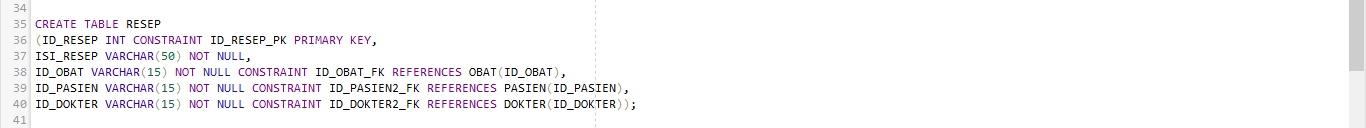
\includegraphics[width=10cm\textwidth]{gambar/7.png}
    \end{center}
    \item Table Diagnosa
    \par Table resep yang mempunyai 6 kolom yaitu id diagnosa, tanggal periksa, hasil diagnosa, id resep, id pasien, dan id-dokter. Pada table ini yang menjadi primary keynya adalah id diagnosa dengan id pasien, id resep, dan id dokter sebagai foreign keynya.
    \begin{center}
    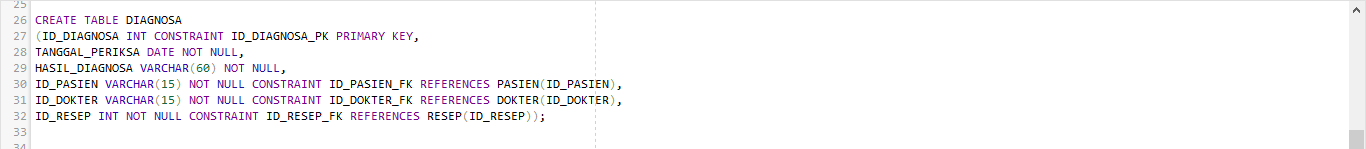
\includegraphics[width=10cm\textwidth]{gambar/8.png}
    \end{center}
    \end{enumerate}
    \item Setelah membuat table maka selanjutnya adalah mengisi baris pada kolom table yang telah dibuat. Berikut adalah cara menambahkan baris pada kolom: 
    \par \begin{enumerate}
        \item Table Pasien
        \par Pada table pasien mempunyai 6 kolom maka baris yang akan dimasukkan juga sebanyak 6 baris sesuai dengan jumlah kolom.
        \begin{center}
    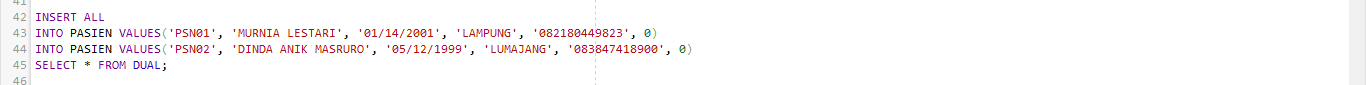
\includegraphics[width=10cm\textwidth]{gambar/9.png}
    \end{center}
    \item Table Dokter
        \par Pada table dokter mempunyai 6 kolom maka baris yang akan dimasukkan juga sebanyak 6 baris sesuai dengan jumlah kolom.
        \begin{center}
    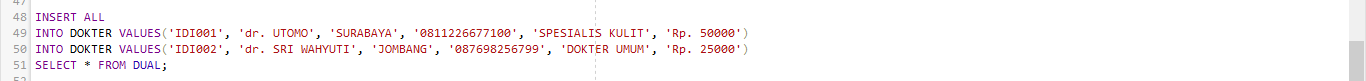
\includegraphics[width=10cm\textwidth]{gambar/10.png}
    \end{center}
    \item Table Obat
        \par Pada table obat mempunyai 4 kolom maka baris yang akan dimasukkan juga sebnayak 4 baris sesuai dengan jumlah kolom.
        \begin{center}
    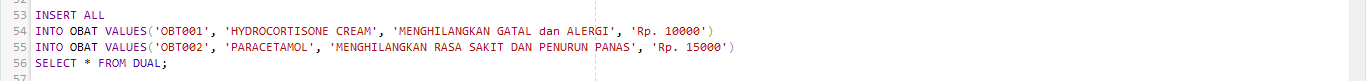
\includegraphics[width=10cm\textwidth]{gambar/11.png}
    \end{center}
    \newpage
    \item Table Resep
        \par Pada table resep mempunyai 5 kolom maka baris yang akan dimasukkan juga sebnayak 5 baris sesuai dengan jumlah kolom. Akan tetapi perhatikan foreign key yang diambil dari table obat,pasien dan juga dokter harus sesuai dengan yang sudah dimasukkan dalam table sebelumnya.
        \begin{center}
    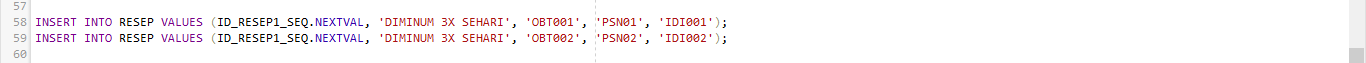
\includegraphics[width=10cm\textwidth]{gambar/12.png}
    \end{center}
    \item Table Diagnosa
        \par Pada table resep mempunyai 6 kolom maka baris yang akan dimasukkan juga sebnayak  baris sesuai dengan jumlah kolom. Akan tetapi perhatikan foreign key yang diambil dari table resep,pasien dan juga dokter harus sesuai dengan yang sudah dimasukkan dalam table sebelumnya.
        \begin{center}
    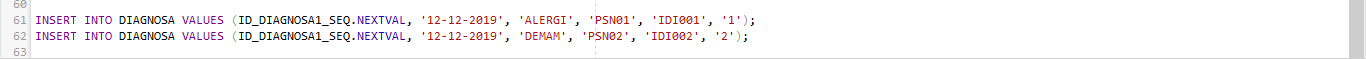
\includegraphics[width=10cm\textwidth]{gambar/13.png}
    \end{center}
    \end{enumerate}
    
    \item Setelah kolo dan baris telah diisi maka selanjutnya adalah pembuatan  fungsi trigger. Fungsi trigger adalah fungsi yang digunakan untuk menampilkan suatu data secara otomatis pada saat insert,delete, dan update pada table. Pada aplikasi ini saya membuat  trigger yang bernama berapa kali periksa, yang mana ketika kita menginsert, mendelete, dan mengupdate pada table Pasien maka yang akan mengalami perubahan secara otomatis pada table Diagnosa  tepatnya di colum tanggal-periksa. Berikut merupakan trigger yang dibuat:
     \begin{center}
    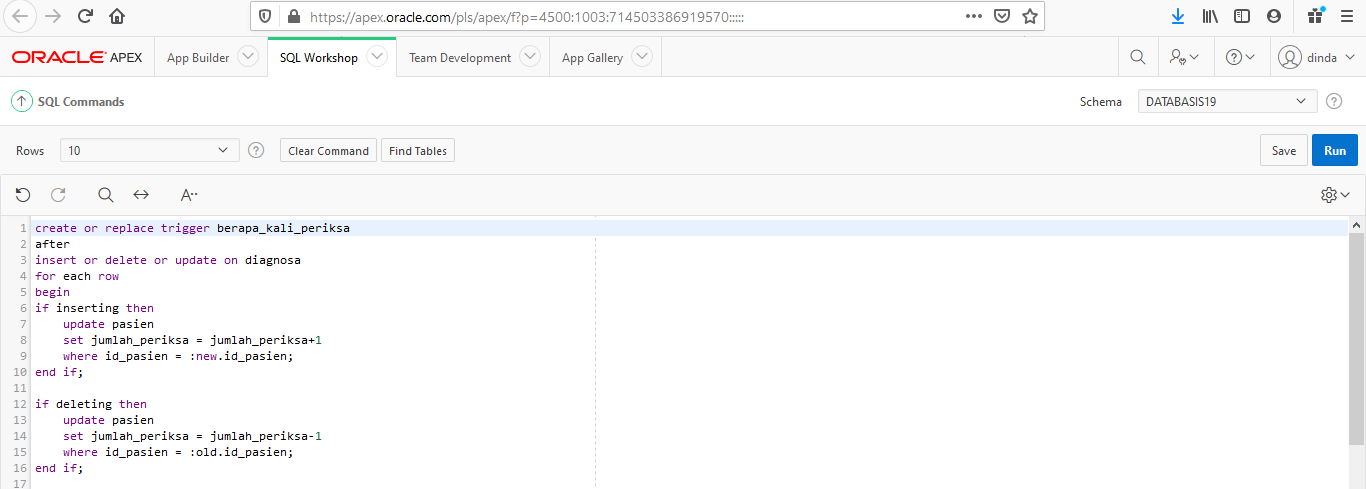
\includegraphics[width=10cm\textwidth]{gambar/14.png}
    \end{center}
    \begin{center}
    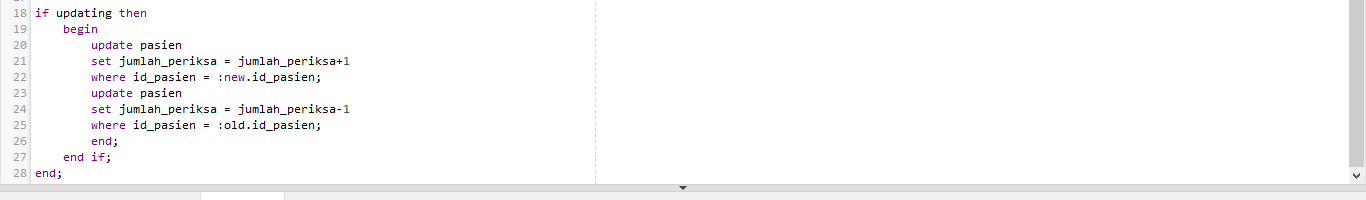
\includegraphics[width=10cm\textwidth]{gambar/15.png}
    \end{center}
    
    \item Setelah itu adalah tahapan membuat view pada aplikasi. View merupakan perintah untuk menggabungkan query join, innerjoin table dengan lebih sederhana. Jadi contoh pada view tersebut akan menampilkan nama pasien, tanggal periksa, dan nama dokter dimana ke-3nya merupakan dari  table yang berbeda. Jadi view lebih menyederhanakan query yang dimasukkan.
    \begin{center}
    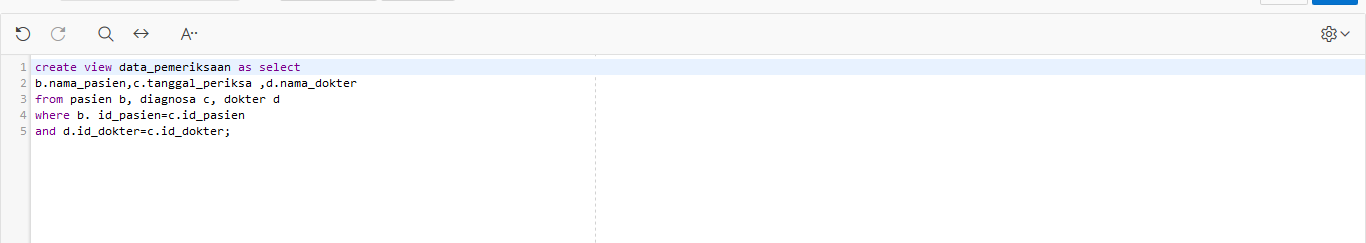
\includegraphics[width=10cm\textwidth]{gambar/16.png}
    \end{center}
    \item Selanjutnya adalah pembuatan sinonim. Sinonim  digunakan untuk memanggil nama table dengan nama yang berbeda. Contohnya table Diagnosa dapat dipanggil dengan nama Pemeriksaan.
    \begin{center}
    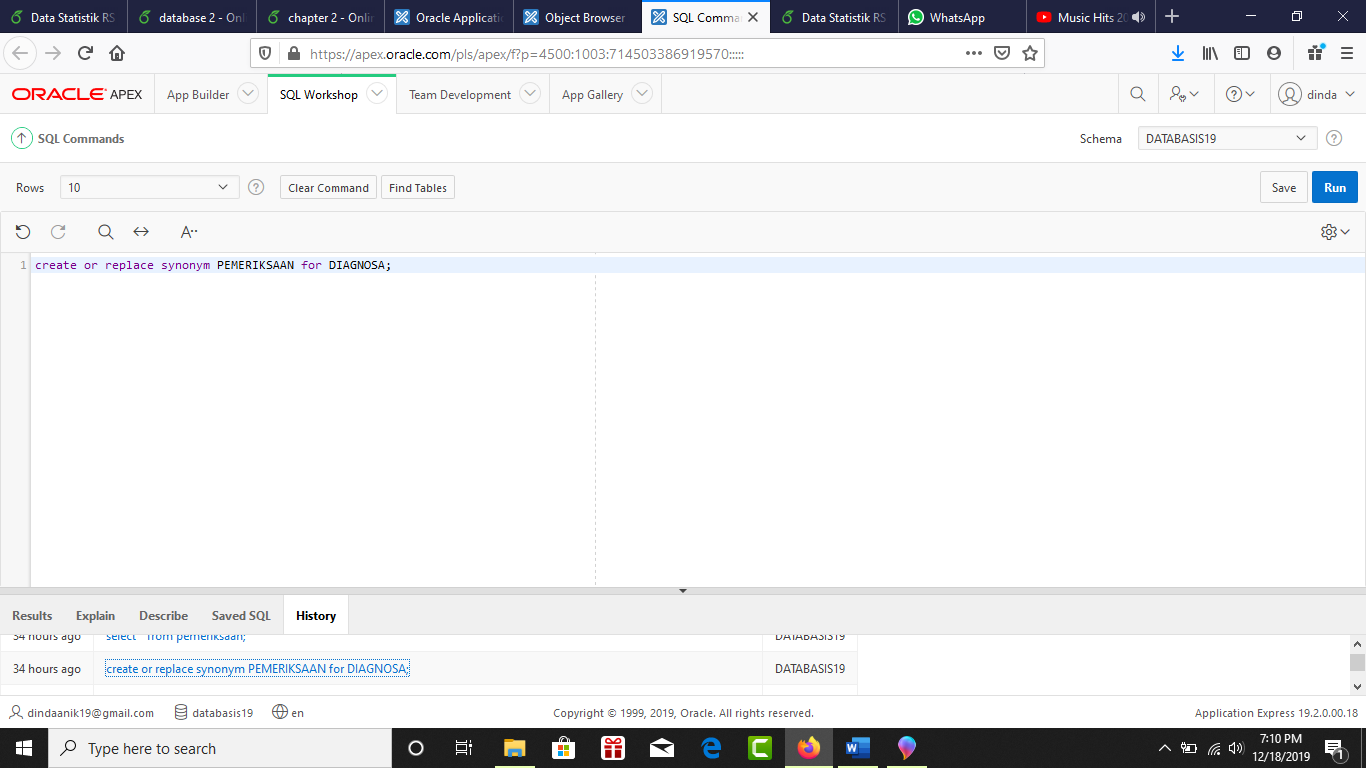
\includegraphics[width=10cm\textwidth]{gambar/17.png}
    \end{center}
    \item Setelah  semuanya selesai, maka selanjutnya adalah pembuatan aplikasi dengan memilih  app builder.
    \begin{center}
    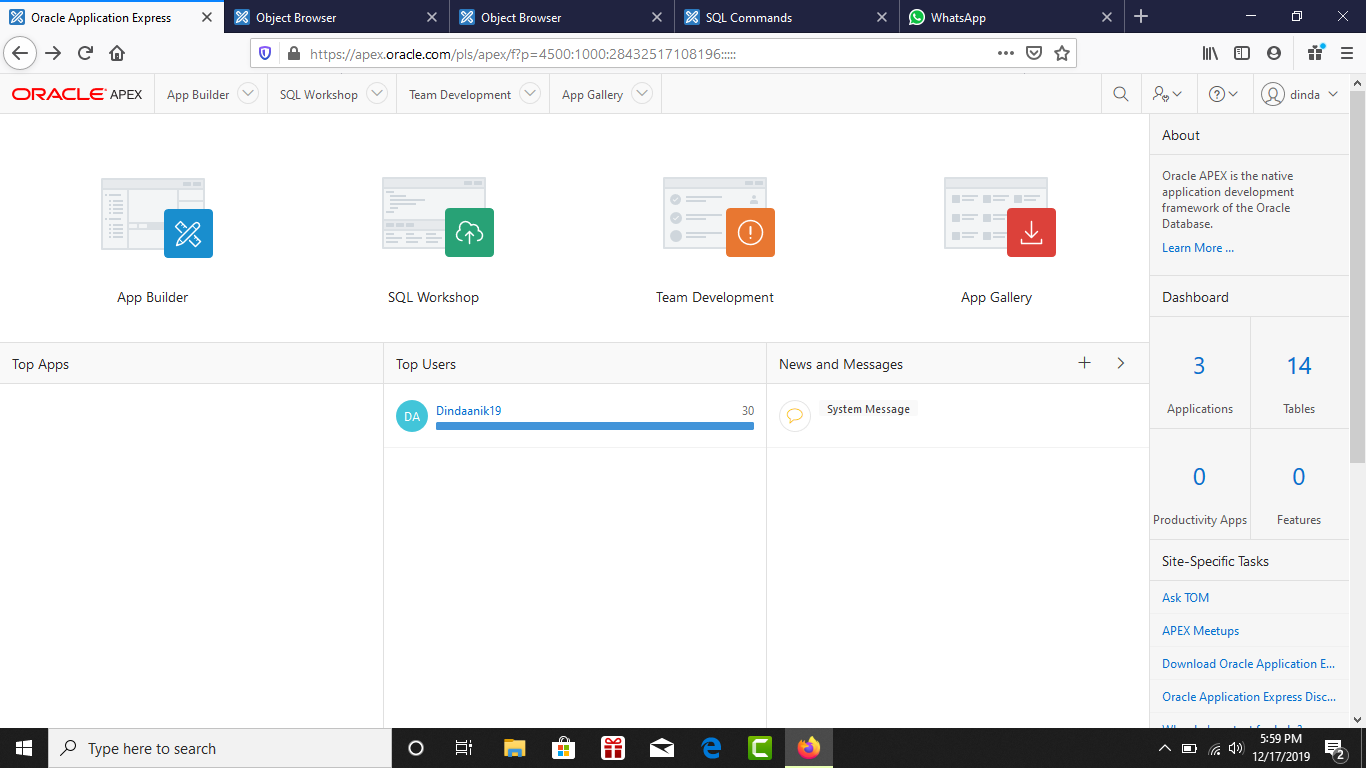
\includegraphics[width=10cm\textwidth]{gambar/18.png}
    \end{center}
    \item Setelah itu pilih create untuk membuat aplikasi yang baru dengan menggunakan data-data yang telah dibuat di oracle apex.
     \begin{center}
    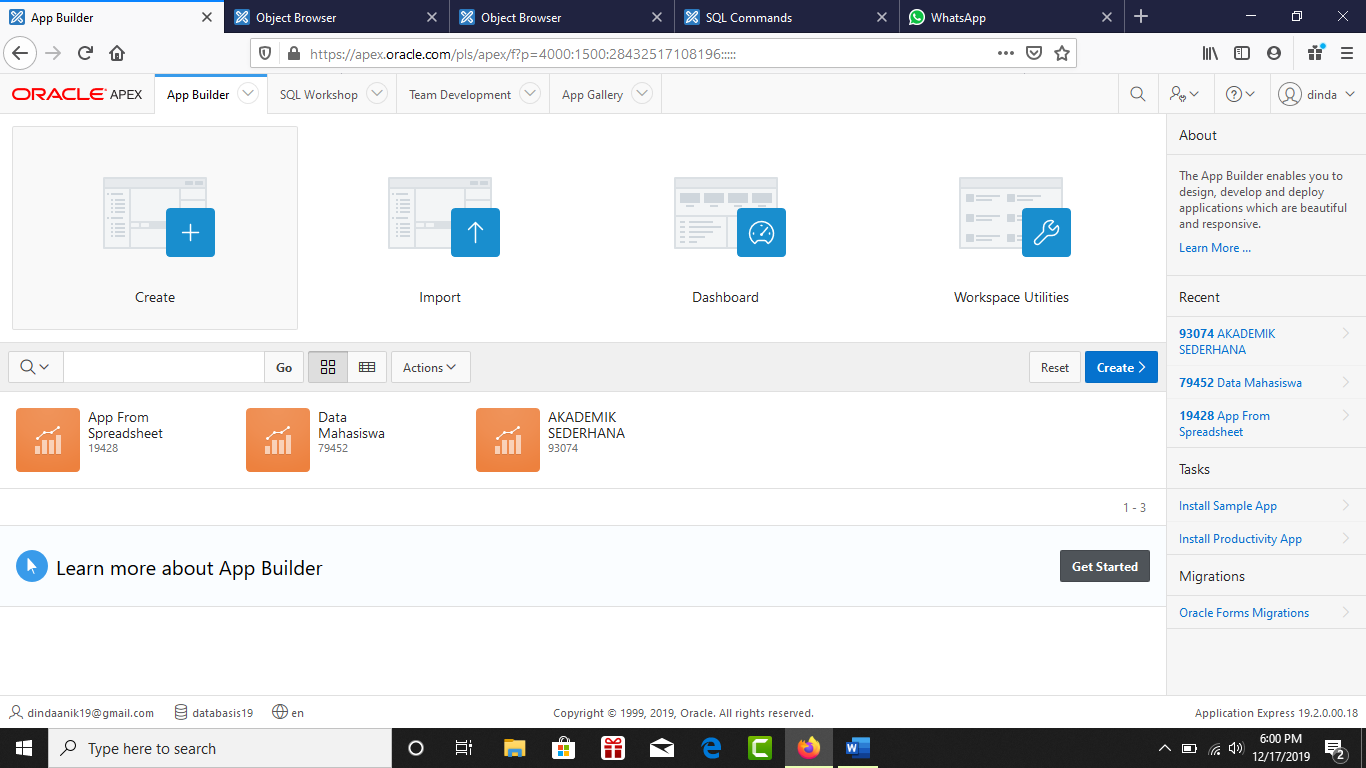
\includegraphics[width=10cm\textwidth]{gambar/19.png}
    \end{center}
    \item Selanjutnya pilih new application yang digunakan untuk membuat aplikasi.
     \begin{center}
    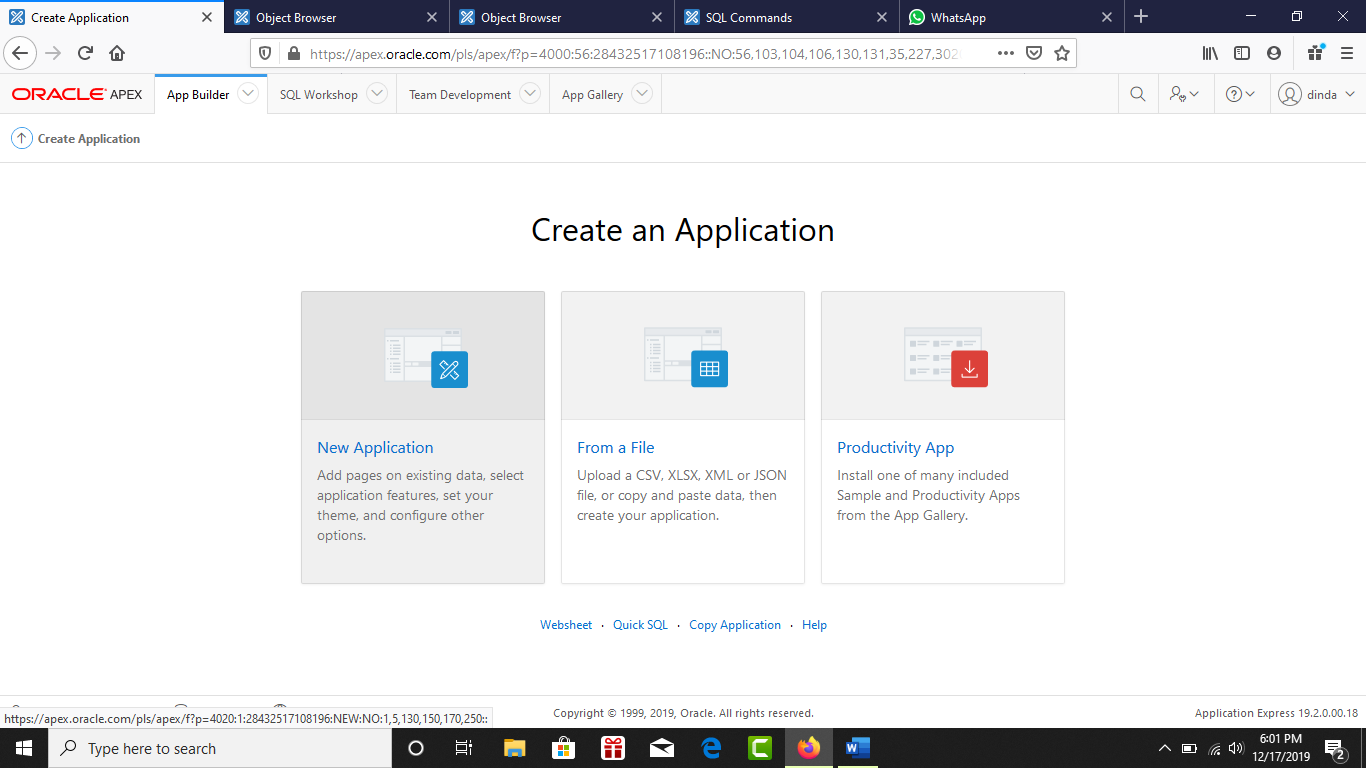
\includegraphics[width=10cm\textwidth]{gambar/20.png}
    \end{center}
    \item Kemudian buatlah nama aplikasi yang akan dibuat,lalu pilih add page untuk memilih page yang akan digunakan untuk membuat aplikasi.
     \begin{center}
    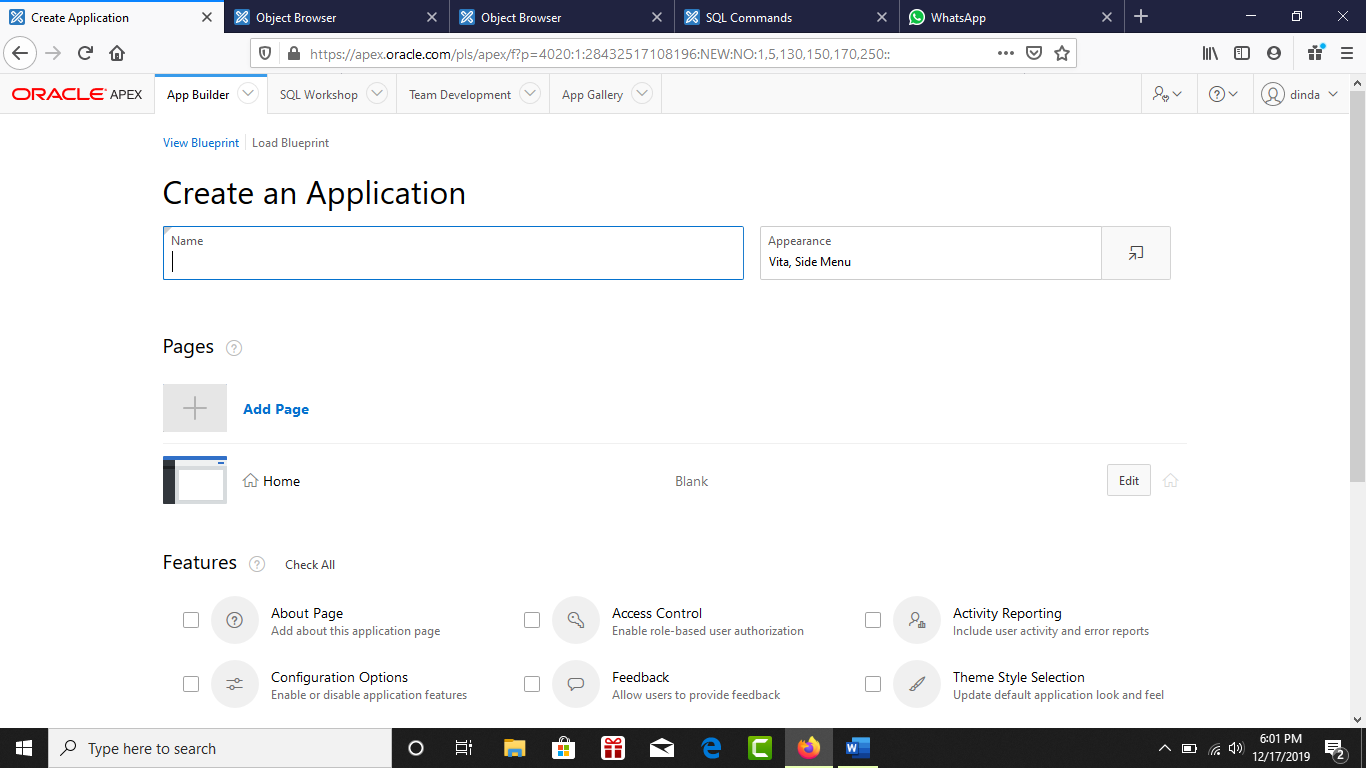
\includegraphics[width=10cm\textwidth]{gambar/21.png}
    \end{center}
    \item Lalu, pilih interactive report untuk page aplikasi yang dibuat.
     \begin{center}
    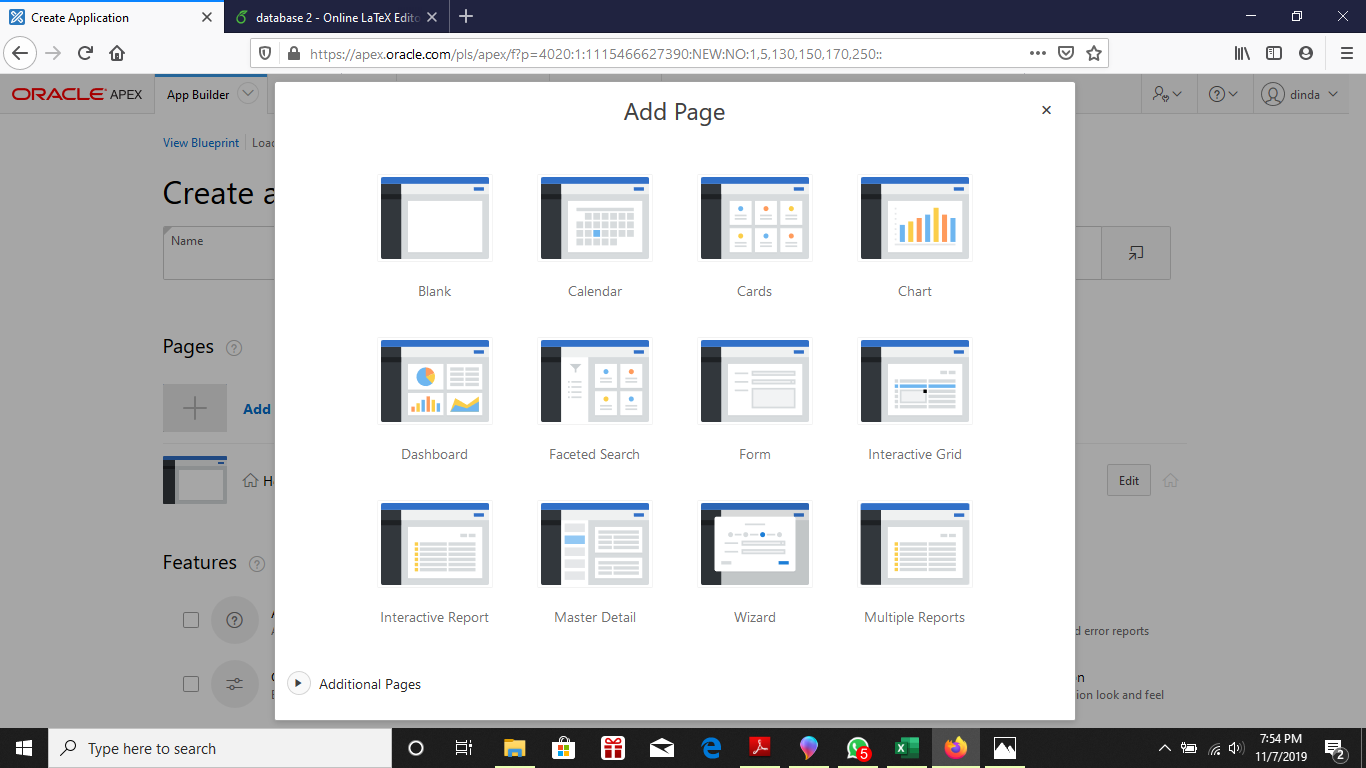
\includegraphics[width=10cm\textwidth]{gambar/22.png}
    \end{center}
    \item Setelah itu page isi page namenya dengan  yang merupakan table yang ingin dibuat pada aplikasi. Pilih table dokter pada table or view lalu add page.
    \begin{center}
    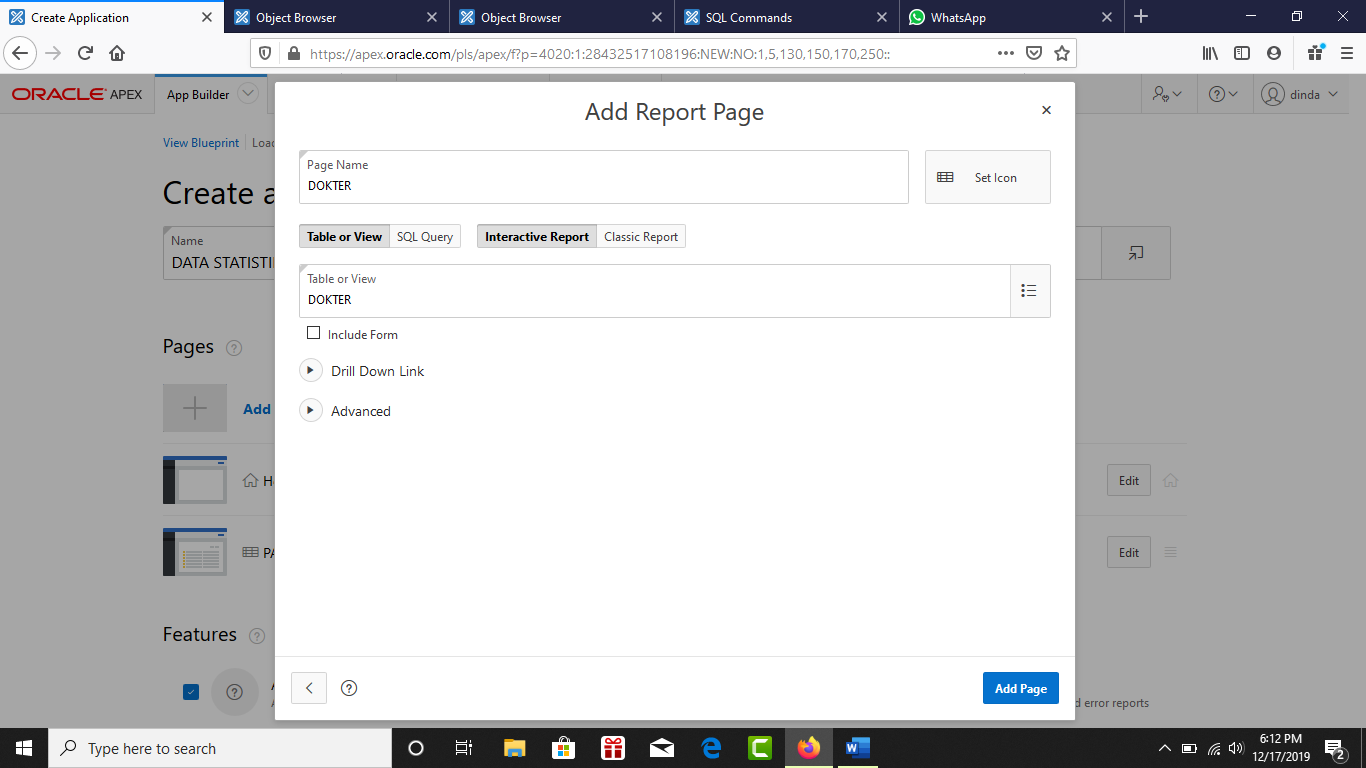
\includegraphics[width=10cm\textwidth]{gambar/23.png}
    \end{center}
    \item lakukan hal yang sama pilih add page dan pilih page intercative report lalu isi name page dengan pasien, dokter, obat, resep, dan diagnosa secara bergantian. Lalu pilih table atau view table yang yang telah dibuat yaitu pasien, dokter, obat, resep, dan diagnosa juga secara bergantian. Jangan lupa jika ingin menambahkan view yang telah dibuat dengan nama hasil panen pada page name lalu pilih view yang telah dibuat yaitu data pemeriksaan. Lalu add page.
    \begin{center}
    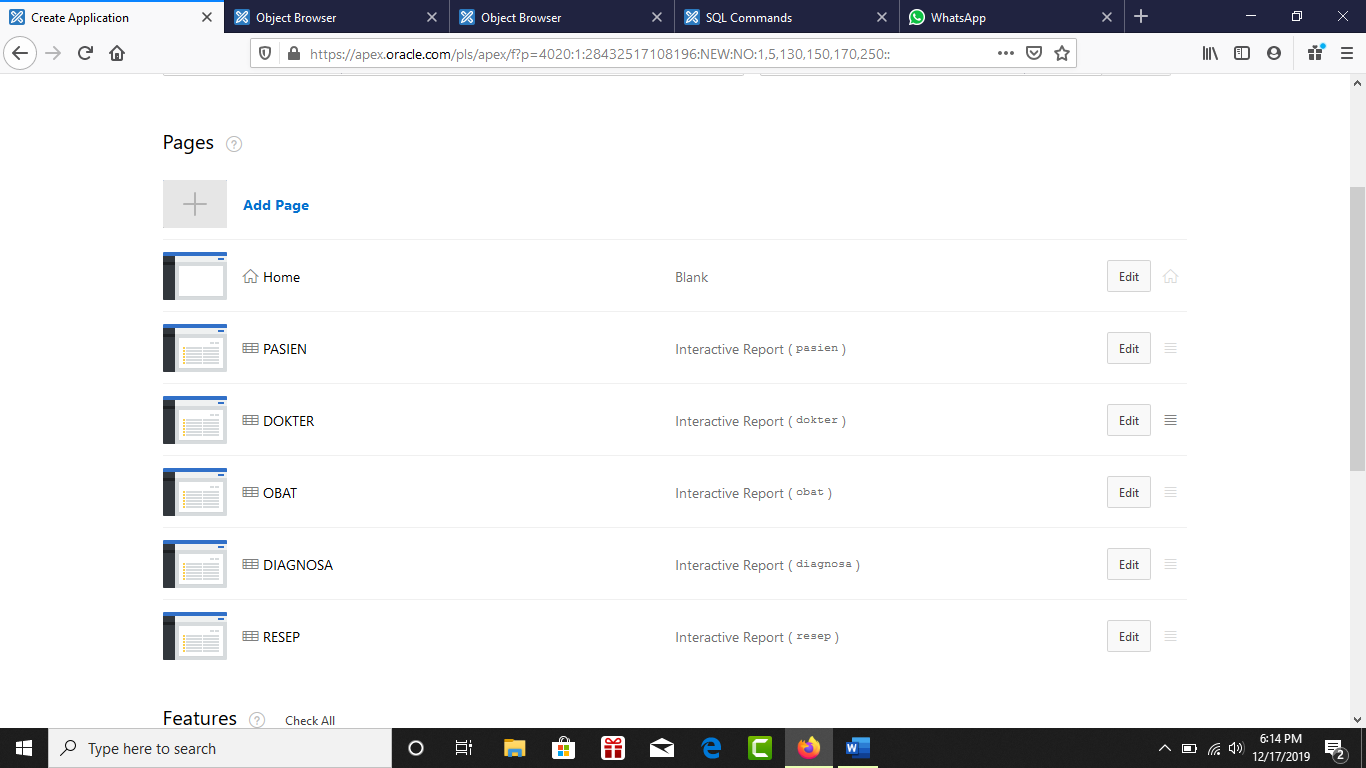
\includegraphics[width=10cm\textwidth]{gambar/24.png}
    \end{center}
    \item Setelah semuanya di add page maka pada features di cek all. Maka setelah itu create application. Tungga hingga selesai.
    \begin{center}
    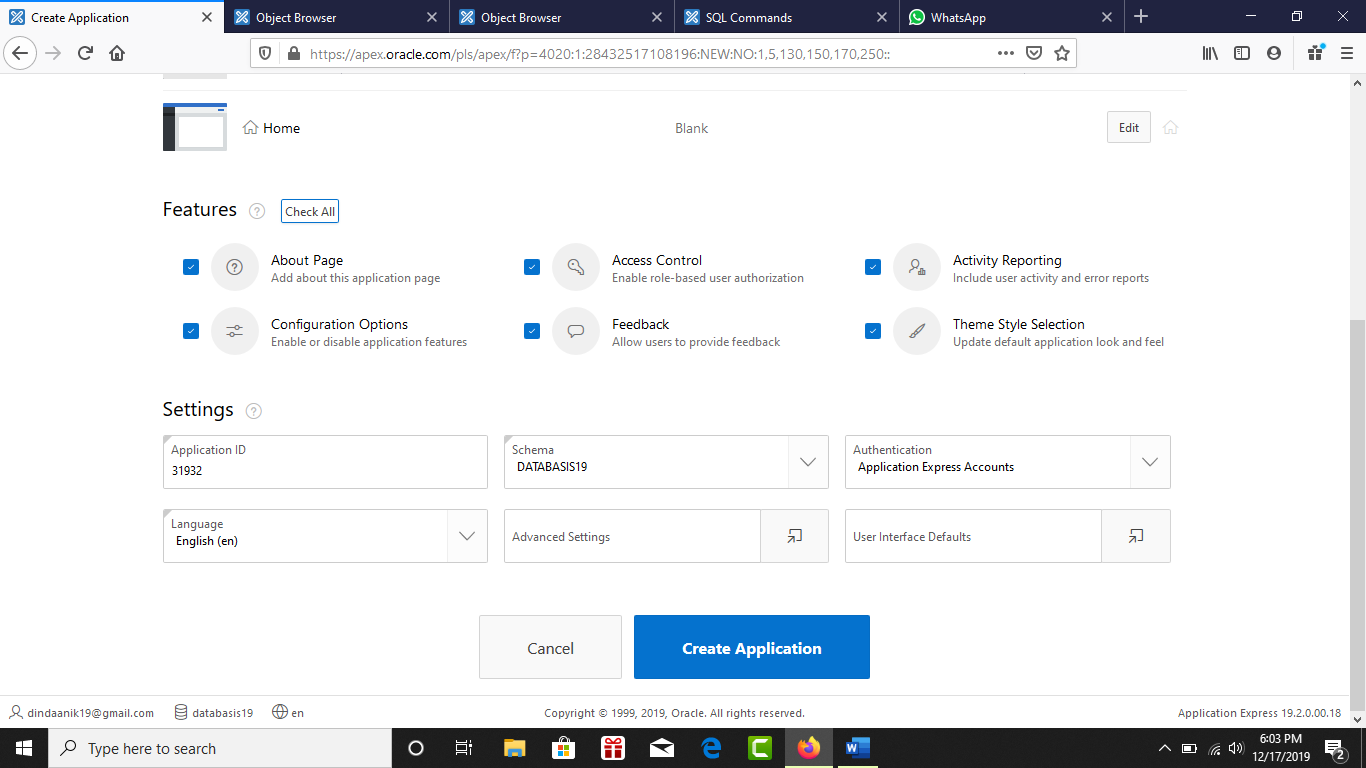
\includegraphics[width=10cm\textwidth]{gambar/25.png}
    \end{center}
    \item Setelah itu pilih run application untuk melihat aplikasi yang sudah dibuat.
    \begin{center}
    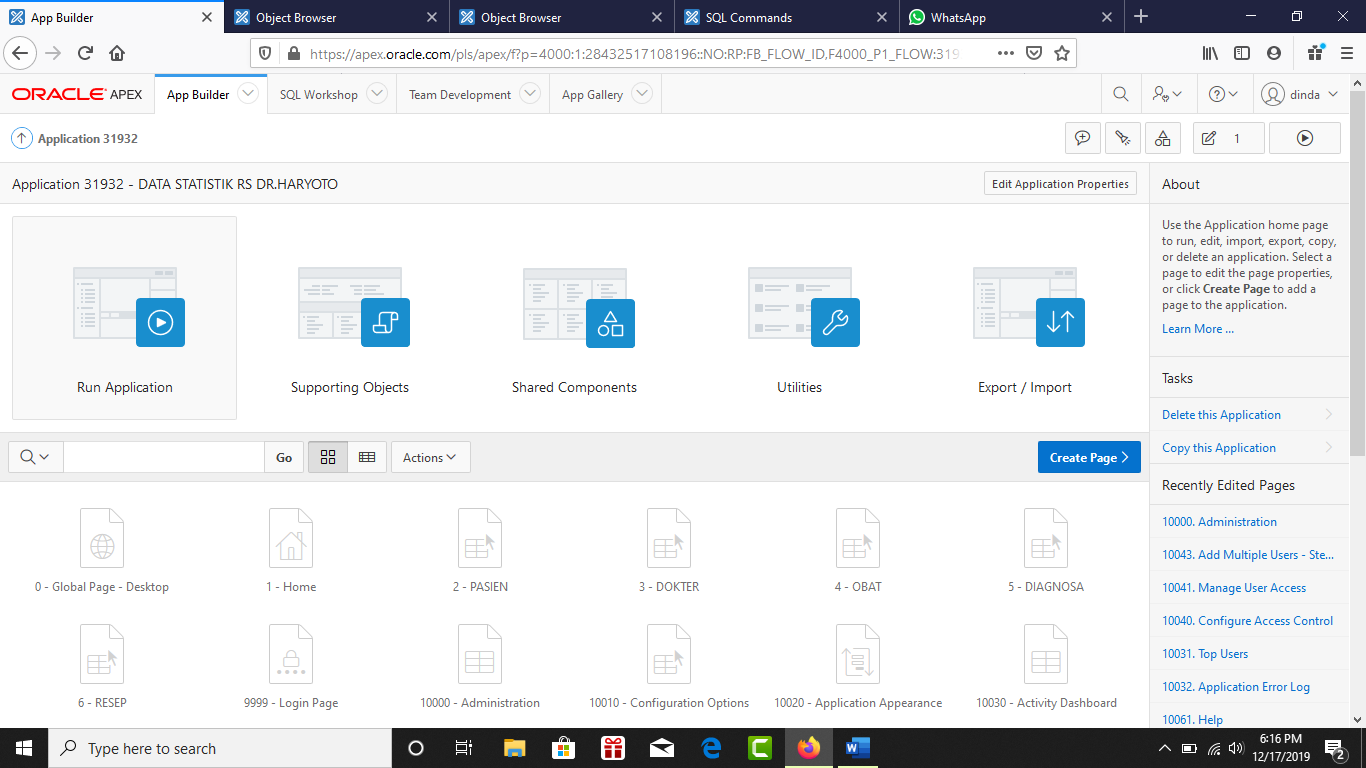
\includegraphics[width=10cm\textwidth]{gambar/26.png}
    \end{center}
    \item Lalu masukkan username dan password untuk melihat aplikasi yang telah dibuat. Lalu sign in
    \begin{center}
    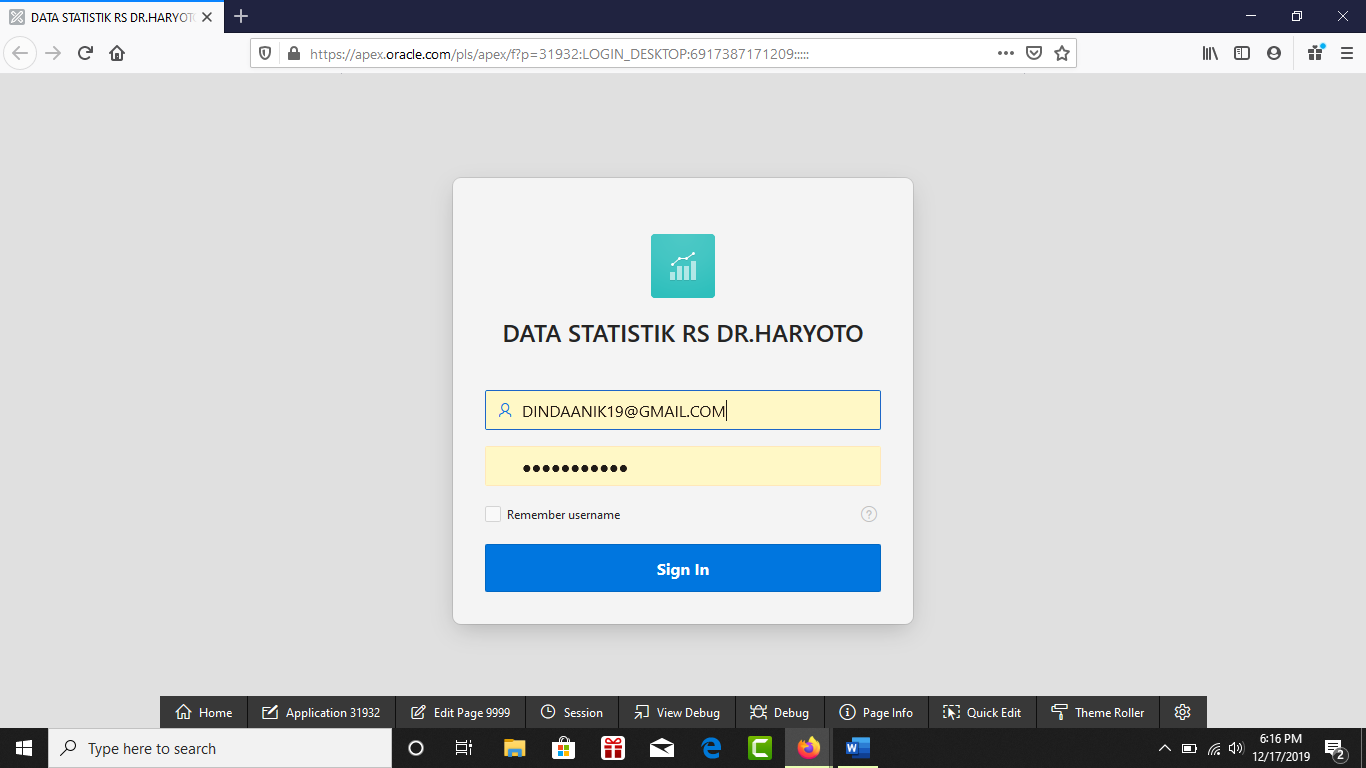
\includegraphics[width=10cm\textwidth]{gambar/27.png}
    \end{center}
    \item Jadi aplikasi data statistik RS dr. Haryoto sudah selesai dibuat
     \begin{center}
    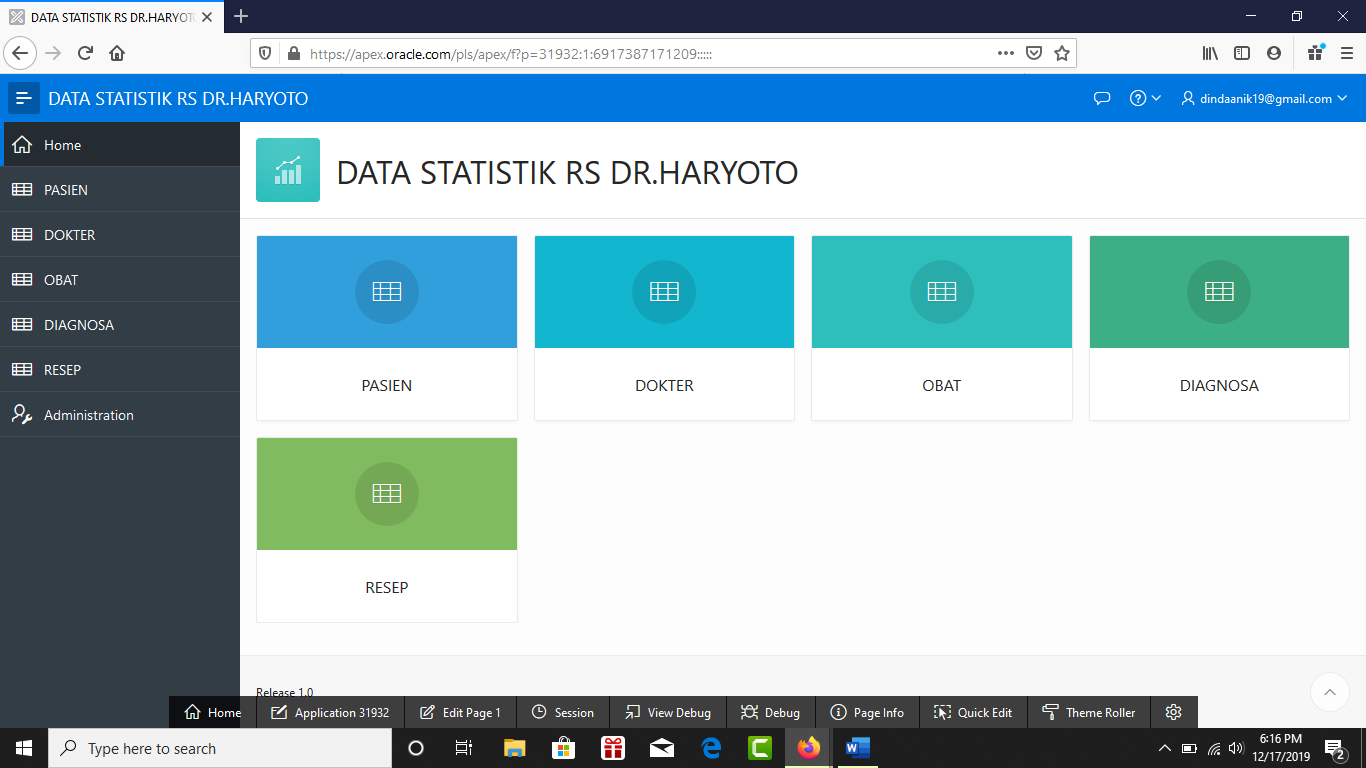
\includegraphics[width=10cm\textwidth]{gambar/28.png}
    \end{center}
\end{enumerate}



        
    